\section{Chapter 3 - Linear Programming}
\usetikzlibrary{arrows,automata}
\subsection{Tuesday 01/28/2025}
\subsubsection{Linear Tricks}
\textbf{Constraint Relaxation: }
If we have the following optimization problem
\begin{align}
  \text{minimize} & \quad c^\top x \\
  \text{subject to} & \quad \sum_j a_j x_j \leq  b
\end{align},
we can relax the constraint by adding a variable $u$ that will allow us to bend the constraint a bit at a cost.
\begin{align}
  \text{minimize} & \quad c^\top x + cost(u) \\
  \text{subject to} & \quad \sum_j a_j x_j - u \leq b
\end{align}

\textbf{Handling Absolute Values: }
Absolute values can be handled by introducing additional variables and constraints.
One way is to split the variable into a positive and negative component.
\begin{align}
  \text{minimize} & \quad c^\top |x| \\
  \text{subject to} & \quad Ax \leq b
\end{align}
Here, we replace $|x|$ with $x^+ - x^-$
\begin{align}
    \text{minimize} & \quad c^\top (x^+ - x^-) \\
    \text{subject to} & \quad Ax \leq b \\
    & \quad x = x^+ - x^- \\
    & \quad x, x^+, x^- \geq 0
\end{align}

\subsubsection{Example Models}
\textbf{Metabolic Flux Balance: } 
A metabolic flux balance problem is a problem where we have a cell that inputs some nutrient and outputs a metabolic yield, the growth of the cell.
We have a $source$ that is an input into a cell $A$ at a rate $v_1$.
$A$ inputs into $B$ at a rate $v_2$.
In parallel, $A$ inputs into $C$ at a rate $v_3$.
B + C input into $2D$ at a rate $v_4$, etc, the rest of the reaction network model is shown below.
\begin{itemize}
    \item $source \to A \quad (v_1)$
    \item  $A \to B \quad (v_2)$
    \item $A \to C \quad (v_3)$
    \item $B + E \to 2D \quad (v_4)$
    \item $source \to E \quad (v_5)$
    \item $B \to C + F \quad (v_6)$
    \item $C \to D \quad (v_7)$
    \item $D \to biomass \quad (v_8)$
    \item $F \to biomass \quad (v_9)$
\end{itemize}

\begin{center}
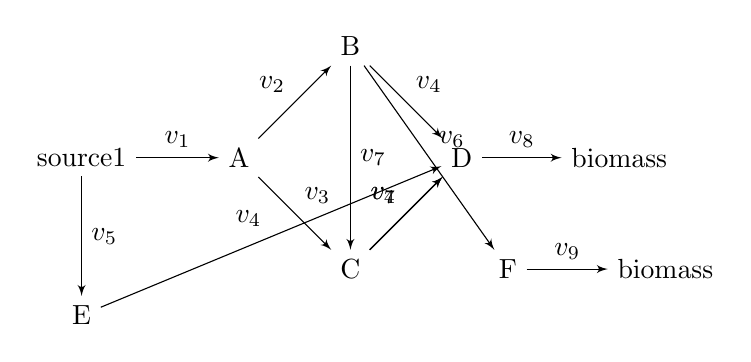
\begin{tikzpicture}[auto, node distance=2cm,>=latex']
    \node [name=source1] {source1};
    \node [right of=source1] (A) {A};
    \node [above right of=A] (B) {B};
    \node [below right of=A] (C) {C};
    \node [below right of=B] (D) {D};
    \node [below of=source1] (E) {E};
    \node [right of=C] (F) {F};
    \node [right of=D] (biomass1) {biomass};
    \node [right of=F] (biomass2) {biomass};

    \draw [->] (source1) -- node {$v_1$} (A);
    \draw [->] (A) -- node {$v_2$} (B);
    \draw [->] (A) -- node {$v_3$} (C);
    \draw [->] (B) -- node {$v_4$} (D);
    \draw [->] (C) -- node {$v_4$} (D);
    \draw [->] (B) -- node {$v_7$} (C);
    \draw [->] (source1) -- node {$v_5$} (E);
    \draw [->] (B) -- node {$v_6$} (F);
    \draw [->] (C) -- node {$v_7$} (D);
    \draw [->] (E) -- node {$v_4$} (D);
    \draw [->] (D) -- node {$v_8$} (biomass1);
    \draw [->] (F) -- node {$v_9$} (biomass2);
\end{tikzpicture}
\end{center}

In this problem, we have an objective we could have multiple goals, one is to maximize the weighted biomass output $w_8 v_8 + w_9 v_9$.
We have constraints that must obey the laws of chemistry and physics. One of them is \textit{mass balance} constraints.
This constraint ensures that the rate of consumption of each edge entering a node is equal to the sum of the rate of production leaving the node.
Flow conservation constraints:
\begin{align}
  \text{maximize} & \quad w_8 v_8 + w_9 v_9 \\
  \text{subject to} & \quad v_1 = v_2 + v_3 \quad (A)\\
  & \quad v_2 = v_4 + v_6 \quad (B)\\
  & \quad v_3 + v_6 = v_7 \quad (C)\\
  & \quad 2v_4 + v_7 = v_8 \quad (D)\\
  & \quad v_5 = v_4 \quad (E)\\
  & \quad v_6 = v_9 \quad (F)
\end{align} 
This problem will be unbounded if we do not constraint the entering sources, so we also introduce \textit{source} constraints.

\textbf{Oil blending}
Consider the problem where we have the following oils with different prices and hardness ratings for each
\begin{itemize}
    \item veg 1 - \$110 - 8.8
    \item veg 2 - \$120 - 6.1
    \item oil 1 - \$130 - 2
    \item oil 2 - \$110 - 4.
    \item oil 3 - \$115 - 5
\end{itemize}
We sell each quantity for \$150.
We have 200 tons of vegetable we can make oil with and 250 tons of non-vegetables we can make oil with.
We want a hardness level between 3 and 6.
To solve this, we can take the vector $\textbf{x} \in \mathbb{R}^5$ as the amount of each liquid $i$ we use. 
We define $\textbf{x}_v$ and $\textbf{x}_n$ subscripts as the subsets of $\textbf{x}$ that are vegetable and non-vegetable.
We similarly define $\textbf{c}$ as the cost vector and $\textbf{h}$ as the hardness vector.
The selling price is $p=150$.
This problem can be formulated as

\begin{align}
  \text{maximize} & \quad 150 (\textbf{1}^\top \textbf{x}) - \textbf{c}^\top \textbf{x} \\
  \text{subject to} & \quad \textbf{1}^\top \textbf{x}_v \leq 200\\
  & \quad \textbf{1}^\top \textbf{x}_n \leq 250 \\
  & \quad 3 (\textbf{1}^\top \textbf{x}) \leq \textbf{h}^\top \textbf{x} \leq 6 (\textbf{1}^\top \textbf{x}) \\
  & \quad \textbf{x} \succeq 0
\end{align}

\subsection{Thursday 01/30/2025}
\subsubsection{Example Models Continued}
\textbf{Oil Blending Over Time}
We now take the oil blending example previously and now consider it over time.
We can buy different raw oil components at different periods of time and store them for use at a later time.
Table \ref{tab:oil_prices} shows the raw oil prices over the next four months
\begin{table}[h!]
\centering
\begin{tabular}{|c|c|c|c|c|c|}
\hline
     & V1  & V2  & O1  & O2  & O3  \\ \hline
M1 & 110 & 120 & 130 & 110 & 115 \\ \hline
M2 & 130 & 130 & 110 & 90  & 115 \\ \hline
M3 & 120 & 110 & 120 & 120 & 125 \\ \hline
M4 & 90  & 100 & 140 & 80  & 135 \\ \hline
\end{tabular}
\caption{Oil prices over time}
\label{tab:oil_prices}
\end{table}

Our storage constraints are that we can store up to 1000 tons of each raw oil each period. 
We start with 500 tons of each oil and must end the total time with 500 tons of each oil.
Going into each period, there is a \$5 cost for holding each ton into the next period.
Our quality constraints are the same, that the total level of hardness must be between 3 and 6. 
Table \ref{tab:oil_hardness} shows the hardness rating of each oil.
Our capacity constraints are that we can not process more than 200 tons of vegetable oil and 250 non-vegetable oil per period. 
\begin{table}[h!]
\centering
\begin{tabular}{|c|c|}
\hline
Oil & Hardness \\ \hline
V1  & 8.8 \\ \hline
V2  & 6.1 \\ \hline
O1  & 2.0 \\ \hline
O2  & 4.2 \\ \hline
O3  & 5.0 \\ \hline
\end{tabular}
\caption{Oil hardness ratings}
\label{tab:oil_hardness}
\end{table}
\\
In order to tackle this problem, we can define the matrix $\Lambda \in \mathbb{R}^{5 \times 5}$  as the cost matrix shown in table \ref{tab:oil_prices}. 
We pad the first row with a 0 vector to represent us starting the first period with inventory.
The matrix $\textbf{X} \in \mathbb{R}^{5 \times 5}$ is our decision variable where each row corresponds to the amount of each oil at the end of each period. 
The first and last column must be equal to a vector of 500s, since we must start and end with 500 of each raw oil.
We also introduce buying and selling variables $\textbf{B} \in \mathbb{R}^{5 \times 5}, \textbf{S} \in \mathbb{R}^{5 \times 5}$ where each row is the amount of an oil we buy and sell before the end of each period.
The first column is $\textbf{0}$ since we can not buy or sell in the 0th period. 
\\
The buying cost component of the objective function is equal to $\textbf{trace}(\Lambda \textbf{X})$.
The inventory holding cost component of the objective function is equal to $5 (\textbf{1}^\top \textbf{X} \textbf{1} - 500 \times 5)$, the $-500 \times 5$ term is to address the fact that we pay no inventory cost for the 0th period.
The selling component of the objective function is equal to $150(\textbf{1}^\top \textbf{S} \textbf{1})$

\begin{align}
  \Lambda = 
  \begin{bmatrix}
    0 & 0 & 0 & 0 & 0 \\
    110 & 120 & 130 & 110 & 115 \\
    130 & 130 & 110 & 90 & 115 \\
    120 & 110 & 120 & 120 & 125 \\
    90 & 100 & 140 & 80 & 135 \\
  \end{bmatrix}
  \quad
  \textbf{X} = 
  \begin{bmatrix}
    500 & x_{11} & x_{12} & x_{13} & 500 \\
    500 & x_{21} & x_{22} & x_{23} & 500 \\
    500 & x_{31} & x_{32} & x_{33} & 500 \\
    500 & x_{41} & x_{42} & x_{43} & 500 \\
    500 & x_{51} & x_{52} & x_{53} & 500 \\
  \end{bmatrix}
  \\
  \textbf{B} = 
  \begin{bmatrix}
    0 & b_{11} & b_{12} & b_{13} & b_{14} \\
    0 & b_{21} & b_{22} & b_{23} & b_{24} \\
    0 & b_{31} & b_{32} & b_{33} & b_{34} \\
    0 & b_{41} & b_{42} & b_{43} & b_{44} \\
    0 & b_{51} & b_{52} & b_{53} & b_{54} \\
  \end{bmatrix}
  \quad
  \textbf{S} = 
  \begin{bmatrix}
    0 & s_{11} & s_{12} & s_{13} & s_{14} \\
    0 & s_{21} & s_{22} & s_{23} & s_{24} \\
    0 & s_{31} & s_{32} & s_{33} & s_{34} \\
    0 & s_{41} & s_{42} & s_{43} & s_{44} \\
    0 & s_{51} & s_{52} & s_{53} & s_{54} \\
  \end{bmatrix}
\end{align}
\\
The objective function is therefore
\begin{align}
  \text{maximize} & \quad 150(\textbf{1}^\top \textbf{S} \textbf{1}) - \textbf{trace}(\Lambda \textbf{X}) - 5 (\textbf{1}^\top \textbf{X} \textbf{1} - 500 \times 5)
\end{align}

